% ===========================================================================
% Section 5: Numerical Studies
% Included under the Numerical Studies section in bdf2-submission.tex. Cross-references
% use labels from the main paper; figure paths are relative to the workspace root.
% Figures: all in figures/ (see \graphicspath in the main file)
% Requires: amsmath, graphicx, booktabs
% REVISION: blue = \new{} rewritten text (content and language); magenta = \torun{} experiments for the authors to run.
% ===========================================================================

\new{We now consider three test problems. Example~1 (Section~\ref{sec:noslip}) is a Taylor--Green vortex with manufactured forcing; we use it for the spatial and temporal convergence, the robustness with respect to $\nu$ and to the pressure, the role of the three CIP terms and the time-step restriction. Section~\ref{sec:vortex3d} shows a three-dimensional travelling vortex computed with a variant of the scheme, and Section~\ref{sec:shear} a deliberately under-resolved shear layer, which shows what the stabilization does to spurious oscillations.}

\new{The experiments use the Scott--Vogelius (SV) pair $P_k/P_{k-1}^{\rm disc}$ on Alfeld-split meshes, which gives pointwise divergence-free velocities, with the Galerkin and the CIP-stabilized method. Where a comparison is informative --- the comparison of the discretizations, the $\nu$-sweep, the pressure-robustness tests, and Sections~\ref{sec:vortex3d} and~\ref{sec:shear} --- we include, as a reference, the inf-sup stable Taylor--Hood (TH) pair $P_k/P_{k-1}$ on standard meshes, which satisfies the divergence constraint only weakly; where stated, it is combined with grad-div stabilization with $\gamma=0.1$~\cite{dFGAJN18}. For SV, grad-div would have no effect, since the discrete velocity is already divergence-free.}

\new{Meshes consist of $n^d$ squares or cubes of size $h=1/n$. Exact and discrete pressures are normalized to zero mean before pressure errors are computed. The time step is given with each example; in Example~1 it is fixed, $\Delta t=5\cdot10^{-3}$, small enough that the temporal error stays below the spatial one on all meshes shown.}
\torun{[Authors: redraw Figures~\ref{fig:vortex3d-h}--\ref{fig:shear-cuts} in the style of the new figures (Computer Modern, ticks and legends 8\,pt, labels 9\,pt): \texttt{print\_figures.py} in galerkit does this from the saved results.]}

\new{To study convergence in time, we fix the mesh and vary the number of steps $N$ on $[0,T]$, so that $\Delta t=T/N$. The temporal error is measured against a reference solution on the same mesh with four times the largest $N$; a second-order method should then show slope $-2$ when the error is plotted against $N$.}

\new{Pressure robustness is tested as in \cite{JLMNR17}: the size of the pressure is varied while the velocity is kept fixed, so a pressure-robust method should produce the same discrete velocity for every pressure. In Example~1 and in the three-dimensional vortex we add $R\nabla\phi$ to the body force, with $\phi=(2\pi)^{-1}\prod_{i=1}^d\sin(2\pi x_i)$, which changes the pressure from $p$ to $p+R\phi$. The gradient part of the force is assembled as $-(R\phi,\nabla\cdot v_h)$, which equals $(R\nabla\phi,v_h)$ for exact integration and vanishes for every divergence-free test function. If the gradient is integrated by quadrature instead, the SV velocity moves by the quadrature error, about $10^{-5}R$ on a coarse mesh; this is not a property of the scheme.}

\new{In all computations the stabilization is normalized by $\max(u_{\min},\|\tu^{n+1}\|_{0,\infty})^{-1}$ with $u_{\min}=10^{-2}$, the variant discussed after \eqref{eq:cip-continuity}, and $\|\tu^{n+1}\|_{0,\infty}$ is evaluated as the maximum over the Lagrange nodes. Experiment (E5) below compares this with the original and the clamped normalization.}

% ---------------------------------------------------------------------------
\new{\subsection{Example 1: Taylor--Green vortex}\label{sec:noslip}
On $\Omega=(0,1)^2$ we consider the generalized Taylor--Green vortex}
\[
\psi(x,y,t)=\pi^{-1}\sin(\pi x)\sin(2\pi y)\,e^{-5\pi^2\nu t},\qquad
u=\nabla\times\psi=e^{-5\pi^2\nu t}
\begin{pmatrix}2\sin(\pi x)\cos(2\pi y)\\[2pt]-\cos(\pi x)\sin(2\pi y)\end{pmatrix},
\]
\new{and compute $f$ from \eqref{eq:strong-form}.}\verify{Taylor--Green setup: confirm the orientation of $\psi$ ($x$ against $y$), the pressure used by the code, and the boundary condition as implemented.} \new{The field satisfies $\nabla\cdot u=0$ and $u\cdot n=0$ on $\partial\Omega$, but its tangential velocity does not vanish there: the computations impose the Dirichlet data of the exact velocity, so this example lies outside the no-slip setting of Theorems~\ref{thm:velocity} and~\ref{thm:pressure} and probes the scheme beyond the letter of the analysis. We have $\|u(t)\|_{0,\infty}=2e^{-5\pi^2\nu t}$, bounded away from zero on $[0,T]$ (Assumption~\ref{ass:lower}), and for small $\nu$ the solution is quasi-steady, with the forcing balancing the genuinely nonlinear convective term. We use $T=0.5$, $\nu=10^{-6}$ unless stated otherwise, SV on the Alfeld split of a crisscross mesh, TH on the crisscross mesh without the split, CIP parameters $(\delta_1,\delta_2,\delta_3)=(10^{-1},10^{-2},10^{-3})$, grad-div parameter $\gamma=0.1$, and $u_h^0$ the modified Stokes projection of $u(0)$. The time step is $\Delta t=5\cdot10^{-3}$ for every mesh.} \verify{CIP weights: every Taylor--Green study records $(\delta_1,\delta_2,\delta_3)=s\,(10^{-1},10^{-2},10^{-3})$, with $\delta_3=\delta_1$ in the reweighted variant of (E4), while the shear-layer runs of Section~\ref{sec:shear} use $s\,(10^{-2},10^{-4},10^{-6})$; the text states the recorded values --- please confirm that the two bases are both intended.}

\new{\paragraph{Without stabilization.} Table~\ref{tab:nostab} shows the two Galerkin discretizations, SV and TH without any stabilization, at $\nu=10^{-6}$. The results are poor: both pairs converge only with orders near $2$ in $L^2$ and near $1$ in $H^1$, below the $h^{k+1/2}$ of the stabilized method, their errors at $n=64$ lie one to two orders of magnitude above the stabilized values below, and TH in addition carries an $O(1)$ divergence error. The remaining experiments quantify what the stabilization adds.}

\begin{table}[htbp]
  \centering\small
  \caption{\new{Example 1, $k=2$, $\nu=10^{-6}$: the unstabilized (Galerkin) methods on all meshes (numbers in brackets: orders between consecutive meshes).}}
  \label{tab:nostab}
  % filled 2026-10-20 from tg.tar: Taylor-Green methods study, unstabilized (Galerkin) runs, k=2, nu=1e-6, all meshes
\begin{tabular}{lrcccc}
\toprule
Method & $n$ & $\|u-u_h\|_0$ & $|u-u_h|_1$ & $\|p-p_h\|_0$ & $\|\nabla\cdot u_h\|_0$ \\
\midrule
SV, Galerkin & 8 & 2.25e-2 & 3.26 & 1.32e-2 & 2e-14 \\
SV, Galerkin & 16 & 6.07e-3 (1.89) & 1.74 (0.90) & 3.95e-3 (1.74) & 4e-14 \\
SV, Galerkin & 32 & 1.53e-3 (1.99) & 0.789 (1.14) & 9.45e-4 (2.06) & 7e-14 \\
SV, Galerkin & 64 & 3.44e-4 (2.16) & 0.298 (1.41) & 2.04e-4 (2.21) & 2e-13 \\
\midrule
TH, Galerkin & 8 & 1.47e-1 & 11.5 & 4.81e-2 & 7.6 \\
TH, Galerkin & 16 & 3.69e-2 (2.00) & 6.13 (0.90) & 9.55e-3 (2.33) & 3.8 \\
TH, Galerkin & 32 & 8.77e-3 (2.07) & 3.06 (1.00) & 2.07e-3 (2.20) & 1.9 \\
TH, Galerkin & 64 & 1.91e-3 (2.20) & 1.40 (1.13) & 4.89e-4 (2.08) & 0.92 \\
\bottomrule
\end{tabular}

\end{table}

\new{\paragraph{(E1) Spatial rates.} Table~\ref{tab:E1} lists, for SV with CIP, the errors at $T$, the stabilization term $(\Delta t\sum_n\Simex^{n+1}(e_h^{n+1},e_h^{n+1}))^{1/2}$ with $e_h=u_h-s_h$, and the discrete $\ell^2(L^2)$ pressure error. Theorems~\ref{thm:velocity} and~\ref{thm:pressure} predict $h^{k+1/2}$ for the velocity and at least $h^{k-1}$ for the pressure. For $k=2$ the stabilization term converges with orders $2.63$, $2.53$, $2.49$ and $2.50$, the predicted $h^{k+1/2}$, and the $L^2$ velocity error with orders $2.50$, $2.69$, $2.84$ and $2.91$, at or above it. The pressure converges with orders between $3.14$ and $2.53$, declining towards the $h^{k+1/2}$ of the velocity and well above the proved $h^{k-1}$ (Remark~\ref{rem:optpressure}). The pressure sum contains the IMEX--Euler starting step, whose error is of order $\Delta t^{3/2}$; the last column omits it. The divergence $\|\nabla\cdot u_h\|_0$ of the SV velocity is below $10^{-13}$ in all runs.} \torun{[Authors: the $k=3$ runs are outstanding; the corresponding rows of Table~\ref{tab:E1} are left open.]}

\begin{table}[htbp]
  \centering\small
  \caption{\new{Example 1, (E1): SV with CIP, $\nu=10^{-6}$. Numbers in brackets: orders between consecutive meshes. ``Stab.'' is $(\Delta t\sum_n\Simex^{n+1}(e_h^{n+1},e_h^{n+1}))^{1/2}$ with $e_h=u_h-s_h$; the last column is the pressure error summed from $n=2$.}}
  \label{tab:E1}
  % filled 2026-10-20 from tg.tar (Afzal setting: T=0.5, nu=1e-6, dt=5e-3 fixed): Taylor-Green rates, SV with CIP
% k=3 runs outstanding -- rows left open.
% k=2, n=64 row: cip study, S1+S2+S3, s=1 -- same scheme/weights; its n=32 record is
% bit-identical to the rates-study n=32 record (all error fields), so this continues the sequence.
\begin{tabular}{rrcccccc}
\toprule
$k$ & $n$ & $\Delta t$ & $\|u-u_h\|_0$ & $|u-u_h|_1$ & Stab. & $\|p-p_h\|_{\ell^2(L^2)}$ & same, $n\ge2$ \\
\midrule
2 & 4 & 5.00e-3 & 8.14e-2 & 2.11 & 0.514 & 2.23e-1 & 2.22e-1 \\
2 & 8 & 5.00e-3 & 1.44e-2 (2.50) & 0.730 (1.53) & 8.32e-2 (2.63) & 2.52e-2 (3.14) & 2.51e-2 (3.14) \\
2 & 16 & 5.00e-3 & 2.22e-3 (2.69) & 0.164 (2.15) & 1.44e-2 (2.53) & 3.47e-3 (2.86) & 3.45e-3 (2.86) \\
2 & 32 & 5.00e-3 & 3.11e-4 (2.84) & 3.54e-2 (2.21) & 2.58e-3 (2.49) & 5.27e-4 (2.72) & 5.24e-4 (2.72) \\
2 & 64 & 5.00e-3 & 4.14e-5 (2.91) & 8.45e-3 (2.07) & 4.57e-4 (2.50) & 9.10e-5 (2.53) & 9.06e-5 (2.53) \\
\midrule
3 & 4 & \torun{--} & \torun{--} & \torun{--} & \torun{--} & \torun{--} & \torun{--} \\
3 & 8 & \torun{--} & \torun{--} & \torun{--} & \torun{--} & \torun{--} & \torun{--} \\
3 & 16 & \torun{--} & \torun{--} & \torun{--} & \torun{--} & \torun{--} & \torun{--} \\
3 & 32 & \torun{--} & \torun{--} & \torun{--} & \torun{--} & \torun{--} & \torun{--} \\
3 & 64 & \torun{--} & \torun{--} & \torun{--} & \torun{--} & \torun{--} & \torun{--} \\
\bottomrule
\end{tabular}

\end{table}

\new{\paragraph{Comparison of the discretizations.} Table~\ref{tab:methods} and Figure~\ref{fig:methods} compare SV and TH, each with Galerkin and CIP, and TH also with grad-div, alone and together with CIP, on $n=8,\dots,64$. SV with CIP is the most accurate discretization on every mesh: at $n=32$ its velocity error lies a factor $2.1$ below TH with CIP and grad-div, $4.6$ below TH with grad-div, and $4.9$ below SV Galerkin, with the gap widening under refinement: at $n=64$ the factors are $2.8$, $9.1$ and $8.3$. CIP acts differently on the two pairs: for SV it reduces the $H^1$ error at $n=32$ by a factor $22$ (from $0.789$ to $3.54\cdot10^{-2}$), while for TH alone the divergence error dominates ($\|\nabla\cdot u_h\|_0\approx1.9$ for Galerkin and $0.52$ with CIP, against $10^{-2}$ with grad-div and $10^{-13}$ for SV), so TH needs grad-div before CIP pays. Figure~\ref{fig:methods} shows the full mesh sequences behind Table~\ref{tab:methods}: the SV with CIP curves correspond to the runs of Table~\ref{tab:E1} (the figure plots the pressure error at $T$, the table its $\ell^2(L^2)$ sum), the unstabilized runs to those of Table~\ref{tab:nostab}.}

\begin{table}[htbp]
  \centering\small
  \caption{\new{Example 1, $k=2$, $\nu=10^{-6}$: errors at $T$ on $n=32$ (numbers in brackets: orders from $n=16$), velocity unknowns $N_{\rm dof}$ and wall-clock time per time step.}}
  \label{tab:methods}
  % filled 2026-10-20 from tg.tar: Taylor-Green methods study, k=2, nu=1e-6, n=32 (orders from n=16)
\begin{tabular}{lrccccr}
\toprule
Method & $N_{\rm dof}$ & $\|u-u_h\|_0$ & $|u-u_h|_1$ & $\|p-p_h\|_0$ & $\|\nabla\cdot u_h\|_0$ & s/step \\
\midrule
SV, Galerkin & 49\,280 & 1.53e-3 (1.99) & 0.789 (1.14) & 9.45e-4 (2.06) & 7e-14 & 3.38 \\
SV, CIP & 49\,280 & 3.11e-4 (2.84) & 3.54e-2 (2.21) & 7.45e-4 (2.72) & 7e-14 & 8.09 \\
TH, Galerkin & 16\,512 & 8.77e-3 (2.07) & 3.06 (1.00) & 2.07e-3 (2.20) & 1.9 & 0.549 \\
TH, CIP & 16\,512 & 1.99e-3 (2.14) & 0.536 (1.09) & 1.61e-3 (2.10) & 0.52 & 2.00 \\
TH, grad-div & 16\,512 & 1.42e-3 (1.78) & 0.247 (0.94) & 1.13e-3 (2.03) & 1.0e-2 & 0.409 \\
TH, CIP + grad-div & 16\,512 & 6.57e-4 (2.45) & 5.55e-2 (1.73) & 1.13e-3 (2.05) & 8.2e-3 & 2.14 \\
\bottomrule
\end{tabular}

\end{table}

\begin{figure}[htbp]
  \centering
  \IfFileExists{figures/ex1_methods_errors.pdf}{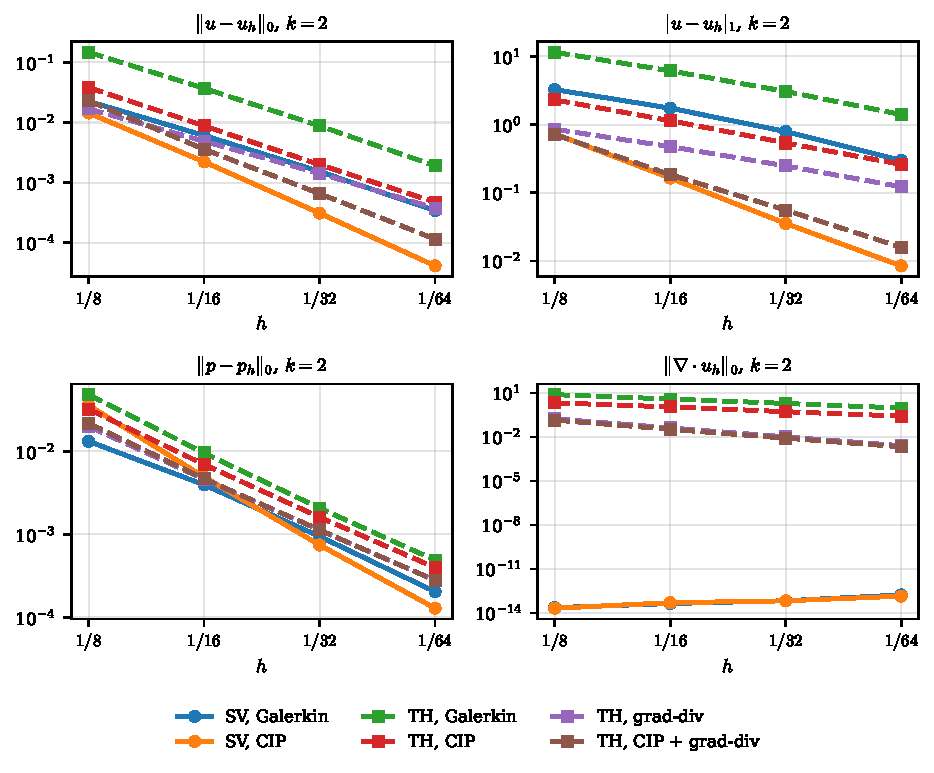
\includegraphics[width=\textwidth]{ex1_methods_errors.pdf}}{\torun{\fbox{\parbox{0.8\textwidth}{\centering\vspace{1cm}[\texttt{ex1\_methods\_errors.pdf}]\vspace{1cm}}}}}
  \caption{\new{Example 1, $k=2$, $\nu=10^{-6}$: velocity and pressure errors and divergence norm at $T$ against $h$ (solid: SV; dashed: TH).}}
  \label{fig:methods}
\end{figure}

\new{\paragraph{Convergence in time.} At $\nu=10^{-6}$ the vortex is quasi-steady and the temporal error is negligible; the time study therefore uses $\nu=0.05$, for which $e^{-5\pi^2\nu t}$ decays by a factor of about $3.4$ over $[0,T]$. On $n=16$ we use $N=10,20,40,80$ and a reference run with $N=320$ on the same mesh (Table~\ref{tab:time}, Figure~\ref{fig:time}). Both SV variants are second order, with velocity orders $2.10$, $2.05$ and $2.09$ and pressure orders $2.15$, $2.09$ and $2.11$ against the reference run; the stabilization leaves the temporal accuracy unchanged, the Galerkin and the CIP values agreeing to three digits.}

\begin{table}[htbp]
  \centering\small
  \caption{\new{Example 1, $k=2$, $n=16$, $\nu=0.05$: temporal error against the reference run with $N=320$ on the same mesh, at the largest $N$, and the observed orders in $N$ between consecutive runs.}}
  \label{tab:time}
  % filled 2026-10-20 from tg.tar: Taylor-Green time study, k=2, n=16, nu=0.05, T=0.5, reference N=320 (SV only in this version)
\begin{tabular}{lcccc}
\toprule
Method & $\|u_h^N-u_h^{\rm ref}\|_0$, $N=80$ & orders & $\|p_h^N-p_h^{\rm ref}\|_0$, $N=80$ & orders \\
\midrule
SV, Galerkin & 2.48e-5 & 2.10, 2.05, 2.09 & 4.58e-6 & 2.15, 2.09, 2.11 \\
SV, CIP & 2.48e-5 & 2.10, 2.05, 2.09 & 4.58e-6 & 2.15, 2.09, 2.11 \\
\bottomrule
\end{tabular}

\end{table}

\begin{figure}[htbp]
  \centering
  \IfFileExists{figures/ex1_time_convergence.pdf}{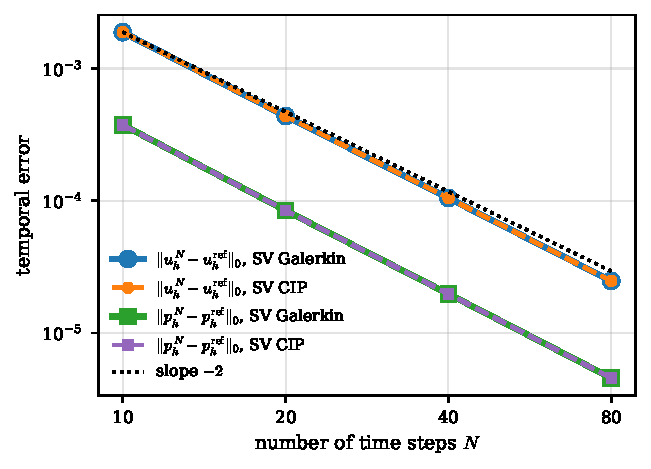
\includegraphics[width=0.62\textwidth]{ex1_time_convergence.pdf}}{\torun{\fbox{\parbox{0.8\textwidth}{\centering\vspace{1cm}[\texttt{ex1\_time\_convergence.pdf}: run \texttt{noslip\_study.py time}]\vspace{1cm}}}}}
  \caption{\new{Example 1, $k=2$, $n=16$, $\nu=0.05$: temporal error of velocity and pressure against the number of steps $N$. The dotted line has slope $-2$.}}
  \label{fig:time}
\end{figure}

\new{\paragraph{(E2) $\nu$-sweep.} Figure~\ref{fig:E2} shows $\|u(T)-u_h^N\|_0$ for $\nu=10^{-1},\dots,10^{-9}$, $k=2$, $n=16$, $32$ and $64$. For SV with CIP the error is bounded uniformly in $\nu$ and saturates at $2.2\cdot10^{-3}$, $3.1\cdot10^{-4}$ and $4.3\cdot10^{-5}$ for $\nu\lesssim10^{-6}$, that is, with orders $2.83$ and $2.87$. SV Galerkin saturates at errors $2.8$, $5.2$ and $9.8$ times larger, and its $H^1$ error ($1.80$, $0.89$ and $0.45$) is $11$ to $53$ times that of SV with CIP ($0.164$, $3.5\cdot10^{-2}$ and $8.5\cdot10^{-3}$). The SV saturation also lies below that of TH with grad-div ($4.90\cdot10^{-3}$, $1.45\cdot10^{-3}$ and $4.04\cdot10^{-4}$) by factors $2.2$, $4.6$ and $9.4$, growing under refinement, while for $\nu\ge10^{-2}$ the discretizations are comparable; the sharper separation appears in the pressure-robustness test (E3).}

\begin{figure}[htbp]
  \centering
  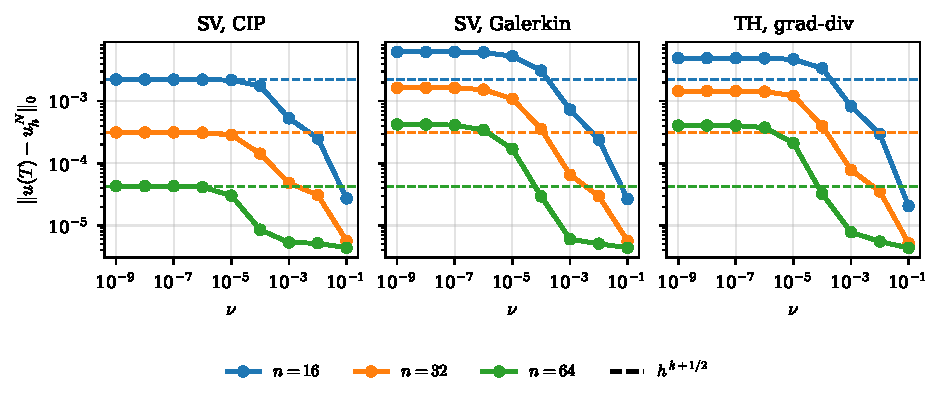
\includegraphics[width=\textwidth]{ex1_nu_sweep.pdf}
  \caption{\new{Example 1, (E2), $k=2$, $T=0.5$: $\|u(T)-u_h^N\|_0$ against $\nu$ on $n=16$, $32$ and $64$, for SV with CIP, SV Galerkin and TH with grad-div. Dashed: $Ch^{k+1/2}$, fitted to SV with CIP on the same mesh.}}
  \label{fig:E2}
\end{figure}

\new{\paragraph{(E3) Pressure robustness.} On $n=32$ with $\nu=10^{-6}$ we add the gradient force $R\nabla\phi$ with $R=10^2,10^4,10^6$ and compare with the run for $R=0$ (Table~\ref{tab:E3}). The SV velocity error is the same to all digits shown for every $R$, and the remaining drift is of order $10^{-11}R$, the solver tolerance applied to a right-hand side of size $R$; the SV pressure error grows in proportion to $\|p+R\phi\|_0$, as it must, while the velocity does not see the pressure. Every TH variant changes in proportion to $R$ or diverges: Galerkin diverges already at $R=10^2$, the stabilized variants carry drifts of order one at $R=10^2$ and of order ten at $R=10^4$, and only CIP with grad-div completes the run at $R=10^6$, with a drift of $2.6\cdot10^2$.}

\begin{table}[htbp]
  \centering\small
  \caption{\new{Example 1, (E3), $n=32$, $\nu=10^{-6}$, $k=2$: drift $\max|u_h^R-u_h^0|$ at $T$ and the velocity error. A dash means that the run diverged.}}
  \label{tab:E3}
  % filled 2026-10-20 from tg.tar: Taylor-Green pressure study, n=32, nu=1e-6, k=2, baseline R=0
\begin{tabular}{lcccc}
\toprule
Method & $R=10^2$ & $R=10^4$ & $R=10^6$ & $\|u-u_h\|_0$, $R=0\to10^6$ \\
\midrule
SV, Galerkin & 6.06e-9 & 2.30e-7 & 1.16e-5 & 1.53e-3 for all $R$ \\
SV, CIP & 6.87e-9 & 1.08e-6 & 5.31e-6 & 3.11e-4 for all $R$ \\
TH, Galerkin & -- & -- & -- & 8.77e-3 at $R=0$ \\
TH, CIP & 1.84 & 13.0 & -- & 1.99e-3 to 4.03 \\
TH, grad-div & 0.547 & 7.11 & -- & 1.42e-3 to 1.87 \\
TH, CIP + grad-div & 0.144 & 2.40 & 2.56e2 & 6.57e-4 to 105 \\
\bottomrule
\end{tabular}

\end{table}

\new{\paragraph{(E4) Role of the three CIP terms.} The analysis needs $S_2$ and $S_3$ only for the recovery step. To see whether they matter in practice, and whether the rate of Theorem~\ref{thm:velocity} survives without them, we run SV with $S_1$ only, $S_1+S_2$ and $S_1+S_2+S_3$, each with $(\delta_1,\delta_2,\delta_3)=s\,(10^{-1},10^{-2},10^{-3})$, $s\in\{0.1,1,10\}$, on $n=8,\dots,64$ (Table~\ref{tab:E4}). With these weights $S_3$ is much weaker than the other terms, so we add $S_1+S_2+S_3$ with $\delta_3=\delta_1$, which raises the third term to the weight of the first. The table also lists the TV ratio $\mathrm{TV}(\omega_h)/\mathrm{TV}(\omega)$ of the vorticity on a $128^2$ grid, the assembly time per step, and the number of nonzeros of the system matrix.}

\new{A geometric scaling $\delta_{j+1}/\delta_j=\beta$ is meant to give the three terms similar weight: each further derivative of a discrete function costs a factor $h^{-1}$, which the extra $h_F^2$ in $S_{j+1}$ cancels, and the factor $\beta$ compensates the larger constants of the higher derivatives; this example uses $\beta=10^{-1}$, the shear-layer runs of Table~\ref{tab:shearcip} use $\beta=10^{-2}$. Table~\ref{tab:E4scaling} checks the choice with the computed values of the terms with unit weights at $T$: a base $\beta$ is balanced when $S_{j+1}/S_j\approx\beta^{-1}$. All three terms couple only the degrees of freedom of the two elements sharing a face, so the stencil of the system matrix stays local; in the shear-layer runs of Table~\ref{tab:shearcip}, activating $S_2$ and $S_3$ fills in about $9\%$ more nonzeros within these blocks than $S_1$ alone ($340\,968$ against $313\,320$ at $n=16$), and $S_3$ adds none beyond $S_2$. In the double shear layer (Section~\ref{sec:shear}, $n=16$, Table~\ref{tab:shearcip}), $S_1$ alone gives TV ratios of $2.00$, $1.11$ and $0.73$ for $s=0.1,1,10$, against $1.87$, $0.96$ and $0.60$ with all three terms, and $S_1+S_2$ and $S_1+S_2+S_3$ agree to $0.01$ in every solution quantity; at $s=1$ and $s=10$, $S_1$ removes the over- and undershoots on its own, while at $s=0.1$ a vorticity undershoot of about $0.1$ remains for every combination of the terms.}

\new{On Example 1 (Table~\ref{tab:E4}), $S_1$ alone is at least as accurate as the full form and converges with the same or higher orders: at $s=1$ and $n=64$, $2.48\cdot10^{-5}$ $(3.14)$ against $4.14\cdot10^{-5}$ $(2.91)$, with the stabilization term of both at the predicted order $2.5$. The reweighted third term ($\delta_3=\delta_1$, a hundredfold increase) stays within a factor of about two of the full form in either direction, so $S_3$ remains numerically inactive at every tested weight; its role is the recovery step in the proof. The measured ratios in Table~\ref{tab:E4scaling} explain this: for the discrete error $e_h$, $S_2/S_1$ reaches $172$--$188$ at $s\ge1$, well above the balanced value $10$ of the base used here, so the second term carries $17$--$19$ times the weighted budget of the first, while $S_3/S_2$ stays between $0.03$ and $0.24$, so with $\delta_3=10^{-3}$ the third term contributes below one percent of the stabilization budget. The number of nonzeros grows by $5\%$ from $S_1$ to $S_1+S_2$ and not at all from $S_2$ to $S_3$, as in the shear-layer runs (Table~\ref{tab:shearcip}), and assembling the full form costs about $4.2$ times $S_1$ alone ($18$\,s against $4.3$\,s per step at $n=64$).}

\begin{table}[htbp]
  \centering\small
  \caption{\new{Example 1, (E4), SV, $k=2$, $\nu=10^{-6}$, $n=64$ (numbers in brackets: orders from $n=32$): CIP terms and strength $s$, $(\delta_1,\delta_2,\delta_3)=s\,(10^{-1},10^{-2},10^{-3})$ for the active terms. ``Stab.'' as in Table~\ref{tab:E1}; TV ratio of the vorticity on a $128^2$ grid; assembly time per step of the convection and CIP matrices.}}
  \label{tab:E4}
  % filled 2026-10-20 from tg.tar: Taylor-Green cip study, k=2, nu=1e-6, n=64 (orders from n=32)
\begin{tabular}{lrccccrr}
\toprule
Terms & $s$ & $\|u-u_h\|_0$ & $|u-u_h|_1$ & Stab. & TV ratio & ms/step & nonzeros \\
\midrule
Galerkin & -- & 3.44e-4 (2.16) & 0.298 (1.41) & -- & 2.02 & 1\,565 & 5\,670\,644 \\
$S_1$ & 0.1 & 1.65e-4 (2.21) & 3.65e-2 (1.40) & 1.05e-4 (2.22) & 1.02 & 4\,563 & 10\,327\,412 \\
$S_1+S_2$ & 0.1 & 1.39e-4 (2.36) & 3.06e-2 (1.63) & 1.72e-4 (2.43) & 1.01 & 7\,784 & 10\,864\,628 \\
$S_1+S_2+S_3$ & 0.1 & 1.40e-4 (2.37) & 3.07e-2 (1.60) & 1.72e-4 (2.43) & 1.01 & 18\,194 & 10\,864\,628 \\
$S_1+S_2+S_3$, $\delta_3=\delta_1$ & 0.1 & 1.50e-4 (2.45) & 3.34e-2 (1.59) & 1.91e-4 (2.70) & 1.01 & 18\,062 & 10\,864\,628 \\
$S_1$ & 1 & 2.48e-5 (3.14) & 8.00e-3 (1.98) & 1.03e-4 (2.48) & 1.00 & 4\,309 & 10\,327\,412 \\
$S_1+S_2$ & 1 & 4.20e-5 (2.91) & 8.59e-3 (2.18) & 4.57e-4 (2.49) & 1.00 & 7\,535 & 10\,864\,628 \\
$S_1+S_2+S_3$ & 1 & 4.14e-5 (2.91) & 8.45e-3 (2.07) & 4.57e-4 (2.50) & 1.00 & 18\,070 & 10\,864\,628 \\
$S_1+S_2+S_3$, $\delta_3=\delta_1$ & 1 & 3.39e-5 (3.22) & 7.54e-3 (2.35) & 5.09e-4 (2.82) & 1.00 & 18\,276 & 10\,864\,628 \\
$S_1$ & 10 & 5.02e-5 (2.70) & 1.09e-2 (1.96) & 2.78e-4 (2.55) & 1.00 & 4\,559 & 10\,327\,412 \\
$S_1+S_2$ & 10 & 1.42e-4 (2.86) & 2.05e-2 (2.15) & 1.44e-3 (2.50) & 1.00 & 7\,744 & 10\,864\,628 \\
$S_1+S_2+S_3$ & 10 & 1.33e-4 (2.86) & 1.89e-2 (2.07) & 1.44e-3 (2.50) & 1.00 & 17\,442 & 10\,864\,628 \\
$S_1+S_2+S_3$, $\delta_3=\delta_1$ & 10 & 2.51e-4 (3.43) & 7.76e-2 (1.44) & 2.43e-3 (2.94) & 1.03 & 18\,311 & 10\,864\,628 \\
\bottomrule
\end{tabular}

\end{table}

\begin{table}[htbp]
  \centering\small
  \caption{\new{Example 1, (E4), $n=64$: ratios of the CIP terms $S_j(w,w)$ with unit weights at $T$, for $w=u_h$ and $w=e_h=u_h-s_h$, in the run with all three terms.}}
  \label{tab:E4scaling}
  % filled 2026-10-20 from tg.tar: Taylor-Green raw S_j(w,w) with unit weights at T, k=2, n=64
\begin{tabular}{rcccc}
\toprule
$s$ & $S_2/S_1$ ($w=u_h$) & $S_3/S_2$ ($w=u_h$) & $S_2/S_1$ ($w=e_h$) & $S_3/S_2$ ($w=e_h$) \\
\midrule
0.1 & 5.3 & 0.24 & 24.7 & 0.08 \\
1 & 36.2 & 0.03 & 172 & 0.03 \\
10 & 46.0 & 0.03 & 188 & 0.03 \\
\bottomrule
\end{tabular}

\end{table}

\new{\paragraph{(E5) Time-step restriction.} With SV and CIP on $n=32$ we vary $\Delta t/h\in\{1/8,1/4,1/2,1,2,4\}$ and compare three normalizations of the stabilization: the original $\|\tu^{n+1}\|_{0,\infty}^{-1}$ of \eqref{eq:fully-discrete-scheme}, the one-sided $\max(10^{-2},\|\tu^{n+1}\|_{0,\infty})^{-1}$ used elsewhere in this section, and the clamped $N_{n+1}^{-1}$ of Remark~\ref{rem:clamp} with $u_{\min}$ half of $\min_t\|u(t)\|_{0,\infty}$ and $U_{\max}=1.25\max_t\|u(t)\|_{0,\infty}$ (Table~\ref{tab:E5}). A run counts as unbounded when $\|u_h^n\|_0$ exceeds $10\|u(t_n)\|_0$. The last column shows the range of $\|\tu^{n+1}\|_{0,\infty}$; the clamp acts only where this range leaves $[u_{\min},U_{\max}]$. No restriction is visible: every run is stable up to $\Delta t=4h$, and the three normalizations give identical errors to all digits shown. The error stays at the spatial level $3.11\cdot10^{-4}$ of Table~\ref{tab:E1} for $\Delta t\le h$ and even drops slightly for the largest steps ($2.20\cdot10^{-4}$ at $\Delta t=4h$), a cancellation within the spatial error level: the solution is quasi-steady at this $\nu$, so the $O(\Delta t^2)$ part is negligible even for the largest step. The range of $\|\tu^{n+1}\|_{0,\infty}$ is $[2.00,2.00]$ throughout --- the exact value $\|u(t)\|_{0,\infty}=2$ reproduced to three digits --- so it never leaves $[u_{\min},U_{\max}]$ and the clamps are never active.}

\begin{table}[htbp]
  \centering\small
  \caption{\new{Example 1, (E5), SV with CIP, $k=2$, $n=32$, $\nu=10^{-6}$: $\|u(T)-u_h^N\|_0$ for the three normalizations of the stabilization.}}
  \label{tab:E5}
  % filled 2026-10-20 from tg.tar: Taylor-Green dt study, SV with CIP, k=2, n=32, nu=1e-6
\begin{tabular}{rcccc}
\toprule
$\Delta t/h$ & original & one-sided & clamped & range of $\|\tilde u_h^{n+1}\|_{0,\infty}$ \\
\midrule
$1/8$ & 3.11e-4 & 3.11e-4 & 3.11e-4 & $[2.00,\,2.00]$ \\
$1/4$ & 3.11e-4 & 3.11e-4 & 3.11e-4 & $[2.00,\,2.00]$ \\
$1/2$ & 3.11e-4 & 3.11e-4 & 3.11e-4 & $[2.00,\,2.00]$ \\
1 & 3.08e-4 & 3.08e-4 & 3.08e-4 & $[2.00,\,2.00]$ \\
2 & 2.85e-4 & 2.85e-4 & 2.85e-4 & $[2.00,\,2.00]$ \\
4 & 2.20e-4 & 2.20e-4 & 2.20e-4 & $[2.00,\,2.00]$ \\
\bottomrule
\end{tabular}

\end{table}

\FloatBarrier

% ---------------------------------------------------------------------------
\subsection{Three-dimensional travelling vortex \new{(a variant of the analysed scheme)}}\label{sec:vortex3d}

\new{The vortex benchmark starts from a radially symmetric swirling flow, which is a steady solution of the incompressible Euler equations~\cite{MajdaBertozzi2002}. By Galilean invariance, the vortex can be carried along by a uniform background velocity $U_0$, as in Gresho's vortex~\cite{GreshoChan1990}. To obtain a Navier--Stokes solution, we move the viscous term into the forcing, $f=-\nu\Delta u$; the velocity--pressure pair is then an exact solution for every $\nu$.}

\new{In all cases the vortex centre starts at $c_0=\tfrac12\mathbf{1}$, the centre of the periodic domain, and moves with constant velocity $U_0$. Relative to the moving centre we use the coordinates}
\begin{equation}\label{eq:vortex}
  \xi_1 = x - \tfrac12 - U_{0,1}\,t, \qquad \xi_2 = y - \tfrac12 - U_{0,2}\,t,
  \qquad r^2 = \xi_1^2 + \xi_2^2,
\end{equation}
\new{where each $\xi_i$ is taken as its nearest periodic image in $[-\tfrac12,\tfrac12)$. The vortex axis is parallel to the $z$-axis, and the axial coordinate enters only through the transport. For a radial profile $g$, the swirl $A\,g(r^2)(-\xi_2,\xi_1)$ is balanced by the pressure gradient $\partial_rp=A^2r\,g(r^2)^2$, which gives an Euler solution; adding the viscous forcing above turns it into a Navier--Stokes solution. The amplitude $A$ is chosen so that the peak swirl speed is one. We take $\nu=10^{-7}$ and integrate up to $T=0.5$. The vortex is transported obliquely across the mesh, convection is of order one, and the pressure is not polynomial, so the test is demanding for all discretizations. The domain is the periodic unit cube, so the no-slip condition of the analysis does not hold; the results illustrate the behaviour of the method rather than test the theorems.}


\new{We stress that the three-dimensional computations in this subsection \emph{do not use the scheme analysed in this paper}: convection is treated fully explicitly, and the stabilization is a single gradient-jump CIP term rather than the three-term form $S$ (see below). Theorems~\ref{thm:stability}--\ref{thm:pressure} therefore do not apply. We include the results because they show pressure robustness and temporal accuracy of SV versus TH in three dimensions; we draw no conclusions about spatial convergence rates from the two SV meshes.}

\new{The three-dimensional test uses a columnar vortex with an axial jet of Batchelor type. Its profile is $q=\max\{0,1-r^2/R^2\}$ with $R=0.45$, $m=5$ and $J=\tfrac12$, the transport velocity is $U_0=(1,\tfrac12,\tfrac14)^\top$, and the amplitude is $A=\bigl(R\,\sigma^{1/2}(1-\sigma)^m\bigr)^{-1}\approx11.87$ with $\sigma=1/(2m+1)$:}
\begin{equation}\label{eq:vortex3d}
\begin{aligned}
  u(x,y,z,t) &= \begin{pmatrix} 1 - A\,\xi_2\,q^5 \\[2pt] \tfrac12 + A\,\xi_1\,q^5 \\[2pt]
                                \tfrac14 + J\,q^5 \end{pmatrix}, \qquad
  p(x,y,z,t) = -\frac{A^2R^2}{22}\,q^{11},\\
  f(x,y,z,t) &= -\frac{20\,\nu\,q^3}{R^2}
                \begin{pmatrix} -2A\,(2-3q)\,\xi_2 \\[2pt] 2A\,(2-3q)\,\xi_1 \\[2pt]
                                J\,(4-5q) \end{pmatrix}.
\end{aligned}
\end{equation}
\new{Since the profile vanishes for $r\ge R$, the field is exactly periodic. It belongs to $H^{m+1/2-\varepsilon}=H^{5.5-\varepsilon}$, and all three velocity components are nonzero.}

\new{For SV we use $P_3/P_2^{\rm disc}$, the lowest admissible degree in three dimensions ($k=d=3$), on Alfeld splits of Kuhn triangulations with $n=2,3,4$. TH uses $P_2/P_1$ on Kuhn meshes with $n=2,4,6,8$.}

\new{The three-dimensional implementation differs from the analysed scheme~\eqref{eq:fully-discrete-scheme} in two ways:}
\begin{itemize}
  \item Convection is treated \emph{fully explicitly}:
        $(({\tilde u}_h^{n+1}\cdot\nabla){\tilde u}_h^{n+1}, v_h)$,
        so the system matrix remains constant in time and no nonlinear solve is needed per step.
  \item The CIP stabilization uses \emph{gradient jumps} across interior facets:
        $\delta\sum_F h_F^2\int_F [\![\nabla u_h]\!]:[\![\nabla v_h]\!]
        \,\mathrm{d}s$, instead of the three-term form $S$.
\end{itemize}
\new{With explicit convection, Theorem~\ref{thm:stability} no longer applies, and the time step is subject to a CFL condition.}

\new{Table~\ref{tab:vortex3d} and Figures~\ref{fig:vortex3d-h}--\ref{fig:vortex3d-pressure} summarize the results.}

\new{Unstabilized SV diverges on the mesh $n=3$, and on $n=4$ its $H^1$ error is $26.7$; with explicit convection, Galerkin SV is simply not usable at this viscosity. SV with CIP ($\delta=10^{-3}$), on the other hand, stays stable on all meshes we tried. From $n=3$ to $n=4$ its observed orders are $2.73$ in $L^2$, $1.59$ in $H^1$ and $2.94$ for the pressure, but two coarse meshes are not enough to say anything about asymptotic rates, and Theorem~\ref{thm:velocity} does not cover this variant anyway. Unstabilized TH also does poorly: $|u-u_h|_1\approx10$ and $\|\nabla\cdot u_h\|_0\approx6$ stay large. The best TH results come from grad-div, which reaches an accuracy per degree of freedom comparable to SV with CIP at this moderate pressure.}

\new{For the temporal tests we use SV on $n=3$ and TH on $n=6$, with $N=40,80,160,320$ and a reference run with $N=1280$. All stabilized methods reach observed orders between $2.0$ and $2.15$ for velocity and pressure, so BDF2 keeps its accuracy in three dimensions as well. The pressure-robustness test (SV on $n=3$, TH on $n=6$) again separates the pairs. The SV velocity changes by at most $2\times10^{-10}$, even for $R=10^6$, where $\|p\|_0\approx5.6\times10^4$. For TH the change grows with $R$: with CIP and grad-div, $\max|u_h^R-u_h^0|$ increases from $6\times10^{-3}$ at $R=1$ to $0.65$ at $R=10^2$, and every TH run diverges for $R\ge10^4$.}

\new{Overall, the three-dimensional results agree with those of Example~1 (Section~\ref{sec:noslip}). They do not, however, show the rate $h^{k+1/2}$: the meshes needed to reach the asymptotic regime are beyond what our direct solvers can handle. Nor do they test the recovery property~\eqref{eq:potential-recovery}, on which the three-dimensional velocity estimate depends (Remark~\ref{rem:velocity}).}

\begin{table}[t]
  \centering\small
  \caption{Travelling vortex, $d = 3$: errors at time $T$
           (numbers in brackets: convergence order with respect to the previous mesh).
           A dash~(--) indicates that the computation diverged.}
  \label{tab:vortex3d}
  \begin{tabular}{lrrccc}
    \toprule
    Method & $n$ & dofs & $\|u-u_h\|_0$ & $|u-u_h|_1$ & $\|p-p_h\|_0$ \\
    \midrule
    SV $P_3$, Galerkin        & 3 &  9\,477 & --            & --            & --            \\
                              & 4 & 22\,464 & 2.0e-1        & 26.7          & 2.1e-1        \\
    SV $P_3$, CIP $10^{-3}$  & 3 &  9\,477 & 1.1e-1 (1.65) & 2.13 (1.07)   & 1.0e-1 (0.99) \\
                              & 4 & 22\,464 & 4.9e-2 (2.73) & 1.35 (1.59)   & 4.5e-2 (2.94) \\
    TH $P_2$, Galerkin        & 8 & 12\,288 & 2.1e-1 (1.73) & 9.80 (0.19)   & 1.2e-1 (1.35) \\
    TH $P_2$, grad-div        & 8 & 12\,288 & 4.2e-2 (2.47) & 1.31 (1.20)   & 4.5e-2 (2.28) \\
    \bottomrule
  \end{tabular}
\end{table}

\begin{figure}[t]
  \centering
  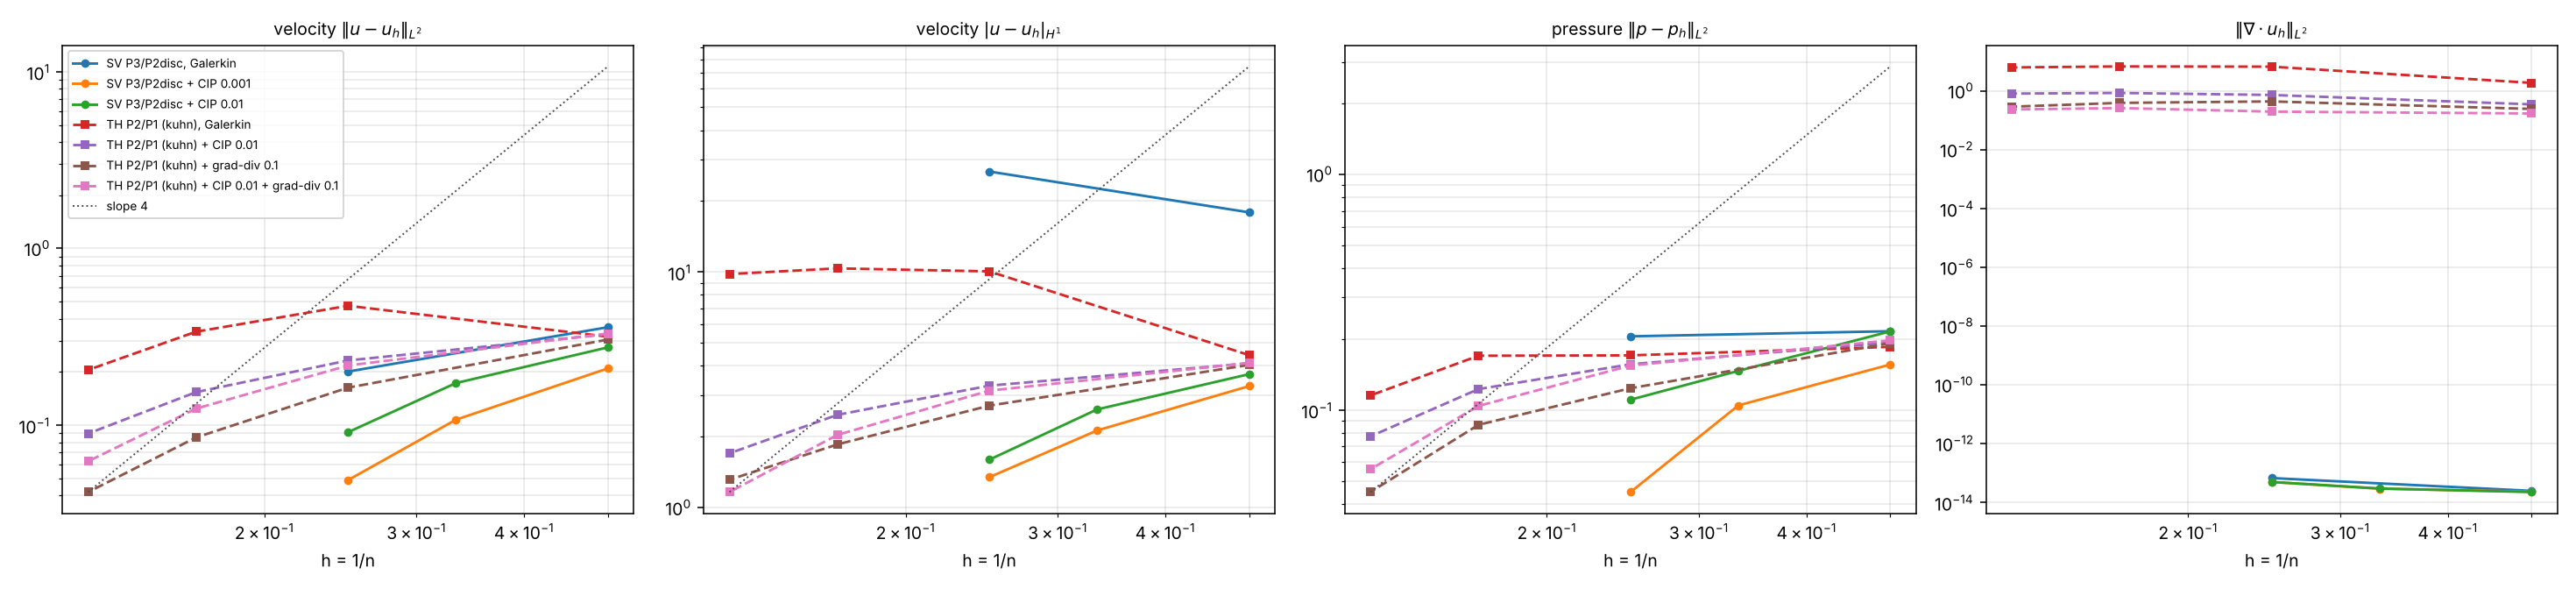
\includegraphics[width=\textwidth]{vortex3d_errors_vs_h.png}
  \caption{Travelling vortex, $d = 3$: errors at time $T$ against $h$
           (solid lines: SV $P_3$; dashed: TH $P_2$).
           The SV Galerkin run on $n = 3$ is absent because it diverged.}
  \label{fig:vortex3d-h}
\end{figure}

\begin{figure}[t]
  \centering
  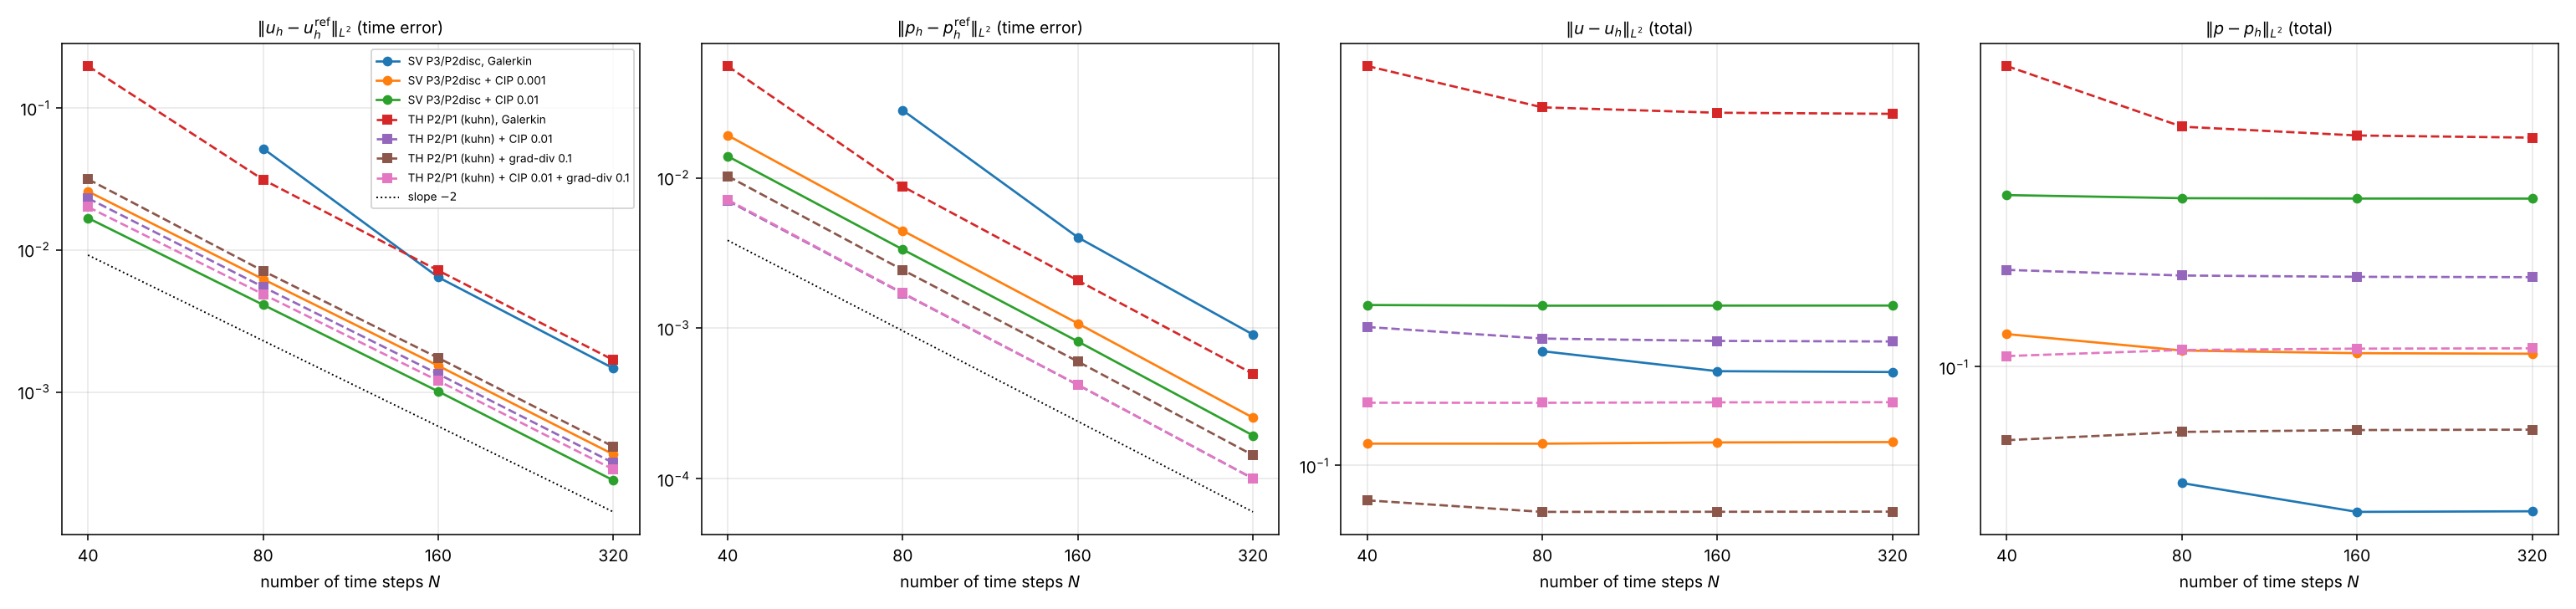
\includegraphics[width=\textwidth]{vortex3d_time_convergence.png}
  \caption{Travelling vortex, $d = 3$: time-discretization convergence against the number of
           steps $N$ (SV at $n = 3$, TH at $n = 6$; temporal error measured as the difference
           from the $N = 1280$ reference run). The dotted line shows slope $-2$.}
  \label{fig:vortex3d-time}
\end{figure}

\begin{figure}[t]
  \centering
  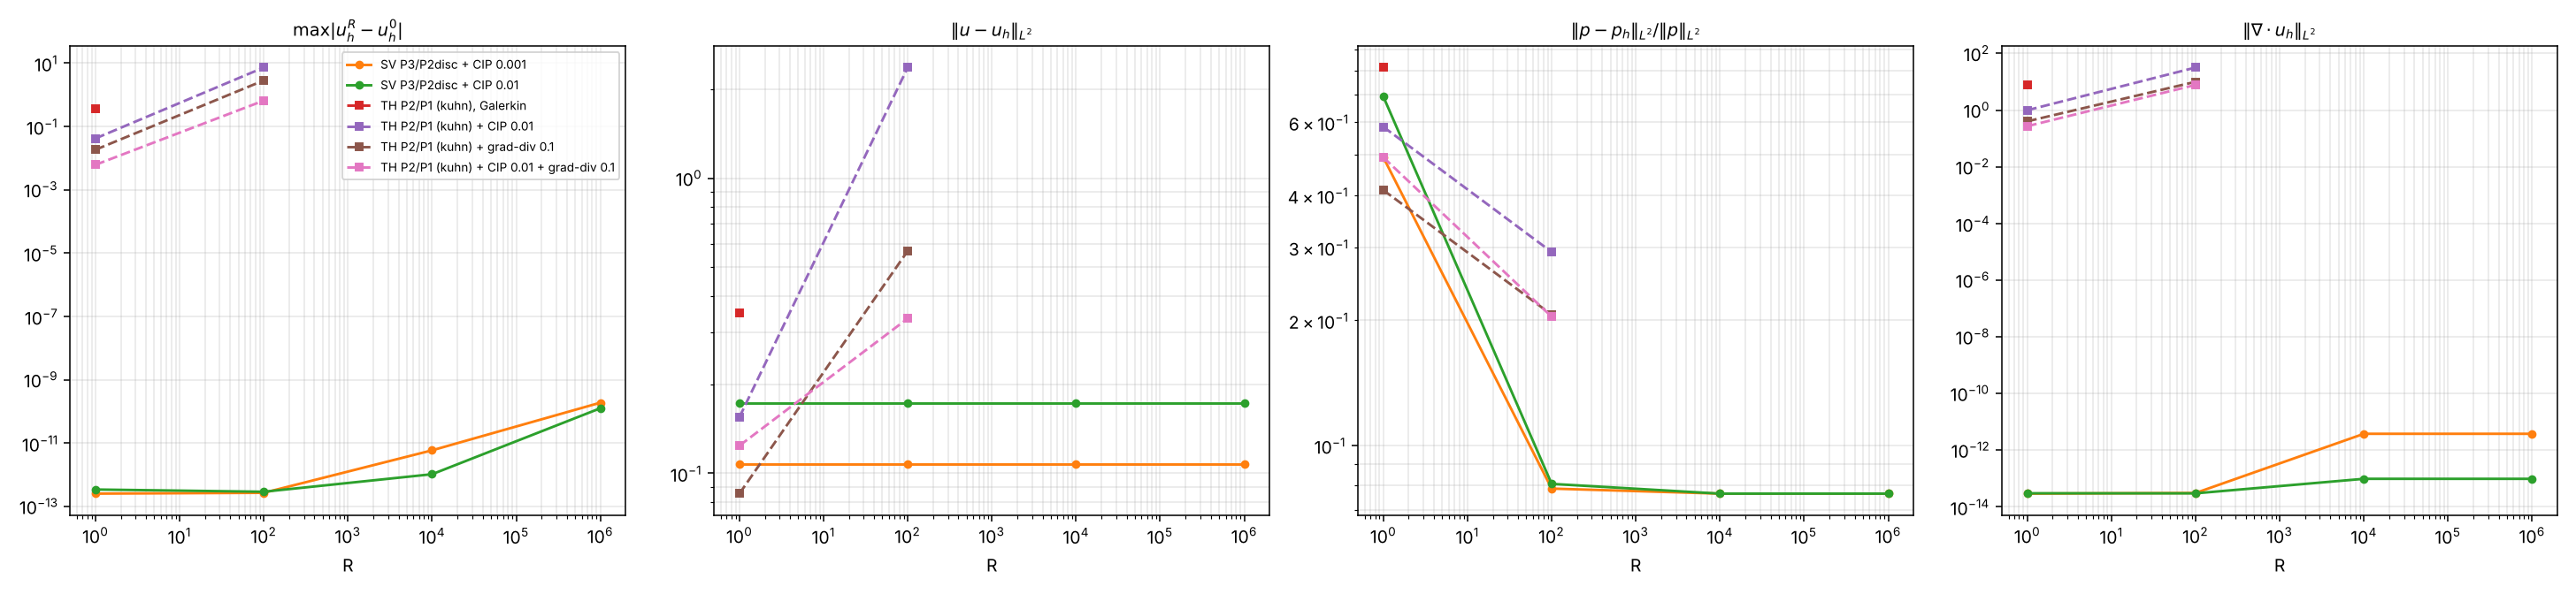
\includegraphics[width=\textwidth]{vortex3d_pressure_robustness.png}
  \caption{Travelling vortex, $d = 3$: pressure robustness
           (SV at $n = 3$, TH at $n = 6$). Missing points indicate divergence.}
  \label{fig:vortex3d-pressure}
\end{figure}

\FloatBarrier

% ---------------------------------------------------------------------------
\subsection{Spurious oscillations in an under-resolved double shear layer}%
\label{sec:shear}

\new{Our last test is the doubly periodic shear layer of Bell, Colella and Glaz~\cite{BellColellaGlaz1989}, a standard benchmark for spotting spurious vortical structures in under-resolved simulations~\cite{BrownMinion1995,MinionBrown1997}. On $(0,1)^2$ the initial velocity consists of two thin shear layers of opposite direction, perturbed by a small sinusoidal mode:}
\begin{equation}\label{eq:shear}
  u_0(x) =
  \begin{pmatrix}
    \tanh\!\bigl(\rho\,(\tfrac{1}{4} - |x_2 - \tfrac{1}{2}|)\bigr) \\[2pt]
    \delta\sin\!\bigl(2\pi(x_1 + \tfrac{1}{4})\bigr)
  \end{pmatrix}.
\end{equation}
\new{We take $\rho=80$, $\delta=0.05$ and $\nu=10^{-4}$. The layers roll up into two large vortices connected by thin braids. On coarse meshes, unstabilized methods tend to produce spurious secondary vortices along the braids, a well-known artefact that makes this problem a good diagnostic~\cite{BrownMinion1995}.}

\new{The reference solution is a fully dealiased pseudo-spectral computation with $512^2$ Fourier modes. We compare SV and TH with $k=2$ on the coarse mesh $n=16$ at $t=1$\new{, and repeat the comparison on $n=32$. Unlike the other tests, the time step here follows a CFL condition, $\Delta t\le0.2/(n\max|u_h^0|)$, rounded so that the output times are multiples of $\Delta t$: $\Delta t=10^{-2}$ on $n=16$ and $\Delta t=1/170\approx5.9\cdot10^{-3}$ on $n=32$}. Oscillations are quantified in two ways: by the overshoots and undershoots of the discrete vorticity $\omega_h$ beyond the reference range, normalized by $\max|\omega_{\rm ref}|$, and by the total variation ratio $\mathrm{TV}(\omega_h)/\mathrm{TV}(\omega_{\rm ref})$. A ratio above one means excess variation, a ratio below one means that the solution is smoother than the reference.}

\new{Unstabilized SV shows strong element-scale oscillations, with a total variation ratio of $4.3$ and a vorticity undershoot of $45\%$. Unstabilized TH is worse still: its total variation ratio is $6.3$, its divergence norm is $\|\nabla\cdot u_h\|_0=41$, and the velocity overshoots by $0.7$. For SV, CIP with unit strength ($s=1$) brings the total variation ratio down to $0.96$ and removes the over- and undershoots. At a tenth of this strength ($s=0.1$) oscillations are still visible, and much stronger CIP smears the vortex cores. For TH, grad-div matters as well: with CIP alone, velocity overshoots of $0.12$ remain, whereas grad-div alone removes the over- and undershoots and gives a ratio of $1.10$. Using both lowers the ratio to $0.74$.}

\new{Even with the oscillations gone, the relative vorticity error stays between $0.74$ and $0.95$ for all stabilized runs. This error is due to the poor resolution of the thin braids on the mesh $n=16$, not to oscillations; no stabilization can recover scales that the mesh cannot represent. \new{On $n=32$ (Table~\ref{tab:shear32}) the ranking is the same and the stabilized vorticity errors drop only to $0.66$--$0.74$, so the braids are still under-resolved. Two details differ: CIP with $s=0.1$ is now the most accurate SV run ($0.66$ against $0.69$ for $s=1$), and grad-div alone leaves a TV ratio of $1.47$ for TH.} We note that the CIP strength $s=1$ in Figure~\ref{fig:shear-showcase} was chosen afterwards, by comparing vorticity errors with the reference; it is a best case, not a recommended parameter value.}

\new{Table~\ref{tab:shearcip} isolates the contribution of the three CIP terms on the mesh $n=16$, for the strengths of experiment (E4) in Section~\ref{sec:noslip}. At $s=1$ and $s=10$, $S_1$ alone removes the over- and undershoots, and at unit strength it brings the TV ratio from $4.30$ down to $1.11$; adding $S_2$ lowers it to $0.97$, and $S_3$ changes no solution quantity by more than $0.01$. The price of the higher-order terms is assembly time: with the transport field, and hence all matrices, changing in every step, $S_1$ takes $52$\,ms per step to assemble, $S_1+S_2$ takes $92$\,ms and the full form $221$\,ms, against $17$\,ms for the Galerkin method. The stabilization is also dissipative: over $[0,1.5]$ the CIP terms account for about $21\%$ of the kinetic-energy loss at $s=0.1$, $35\%$ at $s=1$ and $57\%$ at $s=10$, with the viscous term contributing most of the rest. This over-dissipation at large $s$ is what smears the vortex cores, and it shows in the relative $L^2$ velocity error, which grows from $0.144$ (Galerkin) to $0.258$ ($s=1$) and $0.435$ ($s=10$) while the vorticity error improves.}


\begin{table}[t]
  \centering\small
  \caption{Double shear layer, $k = 2$, $n = 16$, $t = 1$.
           CIP strength $s$ means
           $(\delta_1,\delta_2,\delta_3) = s\,(10^{-2},10^{-4},10^{-6})$.
           The column labelled ``error'' is the relative $L^2$ error of $\omega_h$
           against the spectral reference.}
  \label{tab:shear}
  \begin{tabular}{lccccc}
    \toprule
    Method & TV ratio & $\omega$ over\,/\,under & $u$ over\,/\,under & error & $\|\nabla\cdot u_h\|_0$ \\
    \midrule
    SV, Galerkin           & 4.30 & 0.18\,/\,0.45 & 0\,/\,0       & 1.05 & 2e-10 \\
    SV, CIP $0.1$          & 1.87 & 0\,/\,0.10    & 0\,/\,0       & 0.76 & 2e-10 \\
    SV, CIP $1$            & 0.96 & 0\,/\,0       & 0\,/\,0       & 0.74 & 2e-10 \\
    TH, Galerkin           & 6.31 & 1.10\,/\,1.29 & 0.70\,/\,0.70 & 1.88 & 41    \\
    TH, CIP $1$            & 1.50 & 0\,/\,0.09    & 0.12\,/\,0.12 & 0.95 & 11    \\
    TH, grad-div           & 1.10 & 0\,/\,0       & 0\,/\,0       & 0.82 & 0.46  \\
    TH, CIP $1$ + grad-div & 0.74 & 0\,/\,0       & 0\,/\,0       & 0.79 & 0.46  \\
    \bottomrule
  \end{tabular}
\end{table}

\begin{table}[t]
  \centering\small
  \caption{\new{Double shear layer, $k=2$, $n=32$, $t=1$; columns as in Table~\ref{tab:shear}.}}
  \label{tab:shear32}
  \begin{tabular}{lccccc}
    \toprule
    Method & TV ratio & $\omega$ over\,/\,under & $u$ over\,/\,under & error & $\|\nabla\cdot u_h\|_0$ \\
    \midrule
    SV, Galerkin           & 2.49 & 0.20\,/\,0.38 & 0\,/\,0 & 0.74 & 9e-10 \\
    SV, CIP $0.1$          & 1.52 & 0.17\,/\,0.25 & 0\,/\,0 & 0.66 & 9e-10 \\
    SV, CIP $1$            & 1.02 & 0.01\,/\,0.07 & 0\,/\,0 & 0.69 & 9e-10 \\
    TH, Galerkin           & 3.01 & 0.83\,/\,0.33 & 0\,/\,0 & 0.88 & 7.2   \\
    TH, CIP $1$            & 1.21 & 0.44\,/\,0.01 & 0\,/\,0 & 0.73 & 5.0   \\
    TH, grad-div           & 1.47 & 0\,/\,0       & 0\,/\,0 & 0.73 & 0.20  \\
    TH, CIP $1$ + grad-div & 1.01 & 0\,/\,0       & 0\,/\,0 & 0.74 & 0.16  \\
    \bottomrule
  \end{tabular}
\end{table}

\begin{table}[t]
  \centering\small
  \caption{\new{Double shear layer, SV, $k=2$, $n=16$, $t=1$: role of the three CIP terms, experiment (E4) of Section~\ref{sec:noslip}. CIP strength $s$ as in Table~\ref{tab:shear}; ``$\omega$ error'' and ``$u$ error'' are the relative $L^2$ errors against the spectral reference; ``assembly'' is the time per step for the convection and CIP matrices, ``step'' the total time per step, and ``nnz'' the number of nonzeros of the system matrix.}}
  \label{tab:shearcip}
  \begin{tabular}{lcccccrrr}
    \toprule
    Terms & $s$ & TV ratio & $\omega$ over\,/\,under & $\omega$ error & $u$ error & assembly & step & nnz \\
    \midrule
    Galerkin      & --  & 4.30 & 0.18\,/\,0.45 & 1.05 & 0.144 &  17\,ms & 246\,ms & 178\,152 \\
    $S_1$         & 0.1 & 2.00 & 0\,/\,0.11    & 0.77 & 0.174 &  52\,ms & 316\,ms & 313\,320 \\
    $S_1+S_2$     & 0.1 & 1.88 & 0\,/\,0.10    & 0.76 & 0.176 &  93\,ms & 334\,ms & 340\,968 \\
    $S_1+S_2+S_3$ & 0.1 & 1.87 & 0\,/\,0.10    & 0.76 & 0.176 & 221\,ms & 456\,ms & 340\,968 \\
    $S_1$         & 1   & 1.11 & 0\,/\,0       & 0.75 & 0.265 &  52\,ms & 380\,ms & 313\,320 \\
    $S_1+S_2$     & 1   & 0.97 & 0\,/\,0       & 0.74 & 0.259 &  92\,ms & 385\,ms & 340\,968 \\
    $S_1+S_2+S_3$ & 1   & 0.96 & 0\,/\,0       & 0.74 & 0.258 & 221\,ms & 515\,ms & 340\,968 \\
    $S_1$         & 10  & 0.73 & 0\,/\,0       & 0.81 & 0.383 &  51\,ms & 499\,ms & 313\,320 \\
    $S_1+S_2$     & 10  & 0.61 & 0\,/\,0       & 0.84 & 0.435 &  92\,ms & 481\,ms & 340\,968 \\
    $S_1+S_2+S_3$ & 10  & 0.60 & 0\,/\,0       & 0.84 & 0.435 & 226\,ms & 608\,ms & 340\,968 \\
    \bottomrule
  \end{tabular}
\end{table}

\begin{figure}[t]
  \centering
  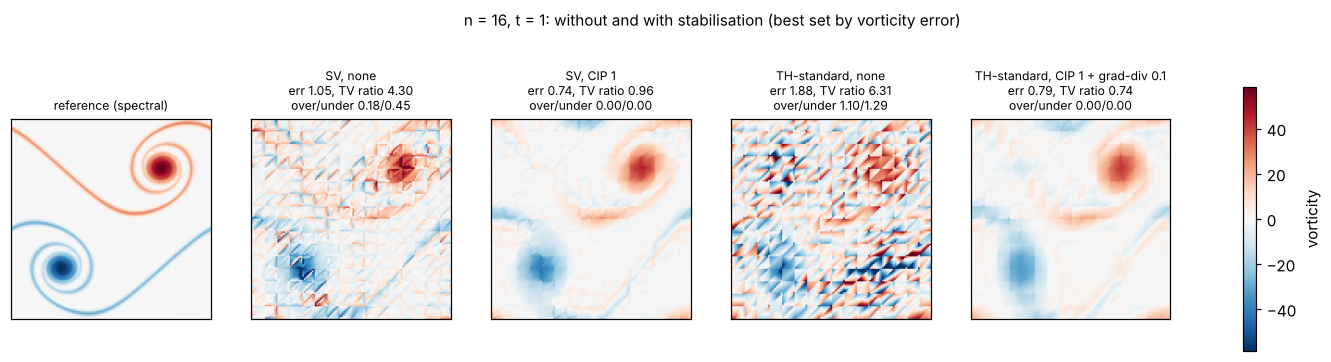
\includegraphics[width=\textwidth]{shear_vorticity_fields_n16.png}
  \caption{Double shear layer: vorticity fields at $t = 1$ on mesh $n = 16$, displayed on a
           common colour scale. From left to right: spectral reference, SV Galerkin, SV with
           the best CIP ($s = 1$), TH Galerkin, and TH with the best stabilization
           (CIP $s = 1$ and grad-div).}
  \label{fig:shear-showcase}
\end{figure}

\begin{figure}[t]
  \centering
  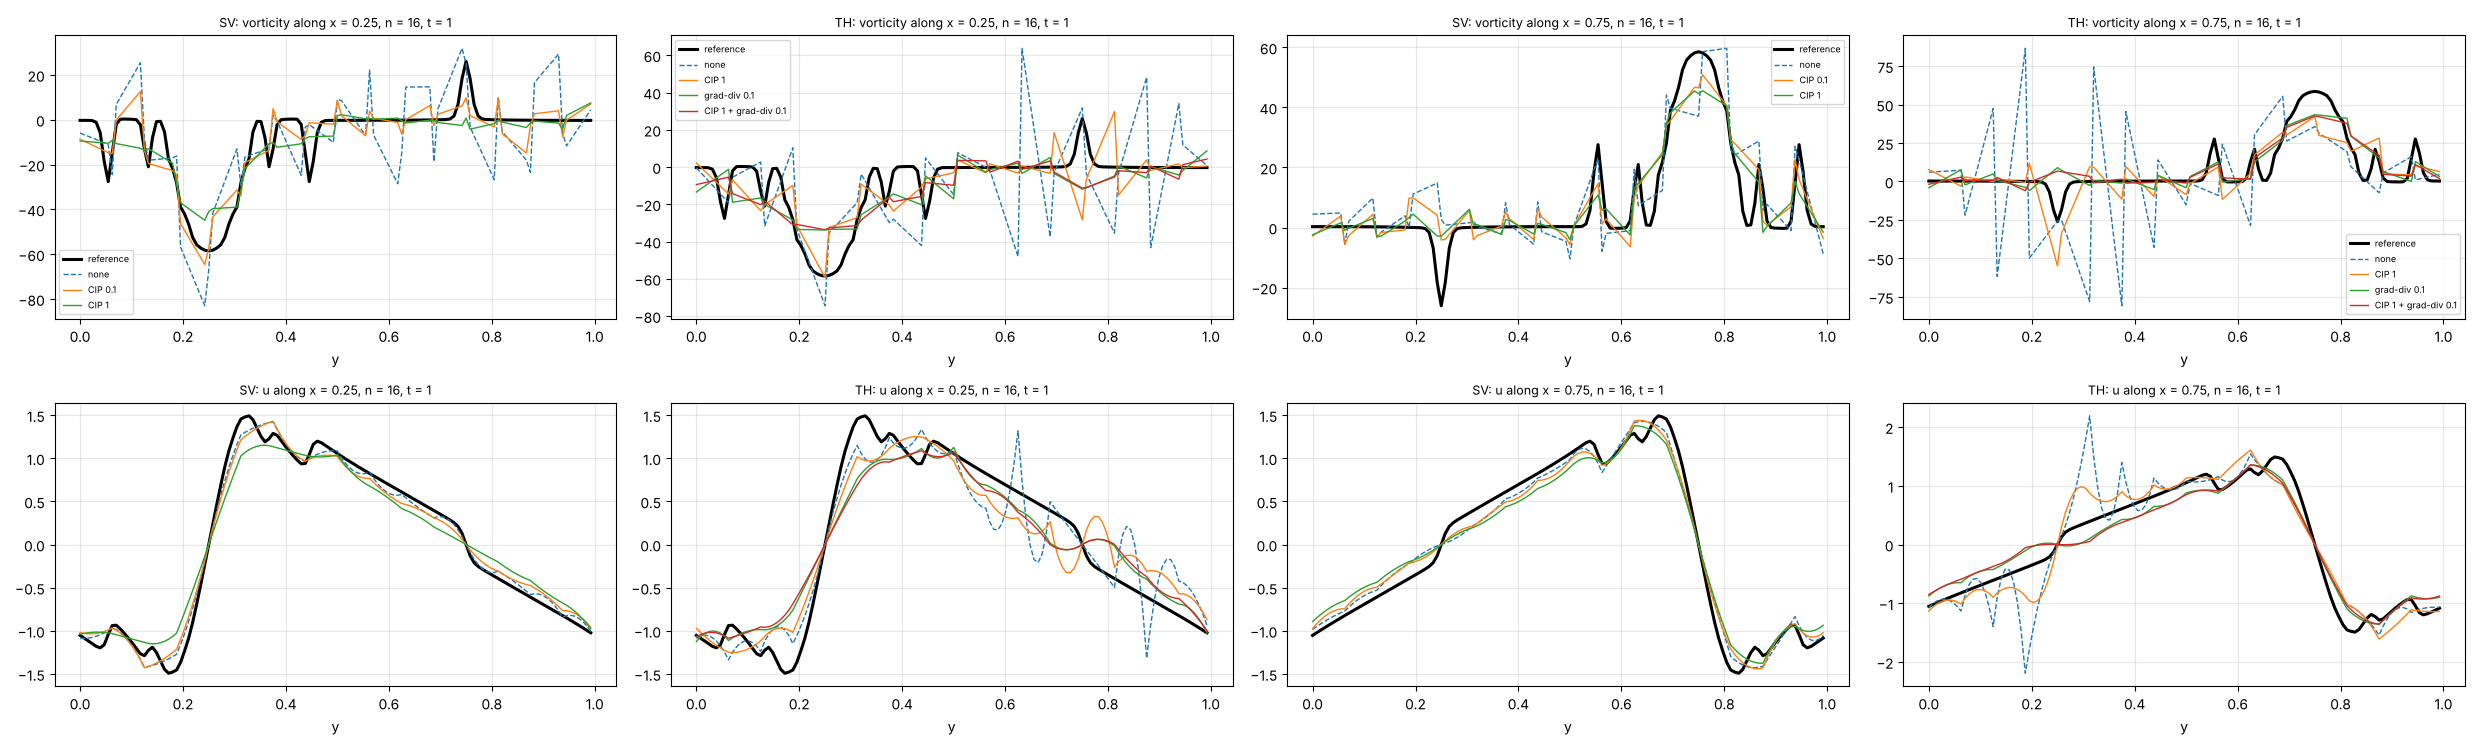
\includegraphics[width=\textwidth]{shear_profiles_n16.png}
  \caption{Double shear layer: one-dimensional profiles of $\omega$ and $u_1$ along the
           vertical lines $x_1 = 0.25$ and $x_1 = 0.75$ at $t = 1$, $n = 16$.}
  \label{fig:shear-cuts}
\end{figure}
\FloatBarrier
